\section{Design}
\label{design}

\subsection{Horizontal Gaze Nystagmus}

Due to the effects of alcohol consumption in the Nystagmus movements, the US police use horizontal gaze Nystagmus as a test, additionally to two others standarized tests (walk and turn and one-leg-stand), to check whether to arrest someone (if they are drunk) or to let them free (if they are sober).The National Highway Traffic Safety Administration of United States wrote a complete guide about the science and usage of Horizontal Gaze Nystagmus for judges, prosecutors and law enforcement \cite{NystagmusTest} in which can be found a deep explanation of the test's performance. Figure \ref{nystagmus} summarizes the parameters the police officer would check if it was an in-person test.

\begin{figure}[H]
    \centering
    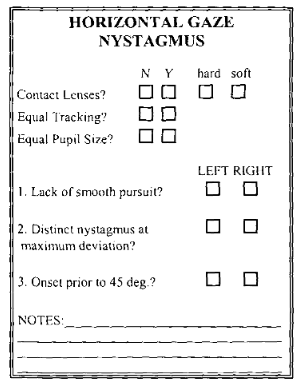
\includegraphics[width=0.5\textwidth]{./img/nystagmus.png}
    \caption{Parameters check by the police officers. Reprinted from \cite{NystagmusTest}.}
    \label{nystagmus}
\end{figure}

To perform this test, the police officer will firstly ask the subject whether they wear lenses and if the answer is positive, whether they are hard or soft. Secondly, they will check that both eyes have an equal tracking of the object, such as a pen or the tip of a penlight, used for the test and the equality of both pupils' size. The use or not of contact lenses, hard or soft, do not affect the test in any way, contrary to some concerns. The lack of equal tracking or equal pupil size may indicate blindness in one eye, a glass eye, a medical disorder or an injury. If the subject exhibits these characteristics, the officer should discontinue the test and may need to seek medical assistance for the individual if a medical disorder or injury appears to exist. After these checks, the test starts with three different clues (each of the subtests performed to check the gaze): lack of smooth pursuit, distinct nystagmus at maximum deviation and onset prior to 45 degrees. These three clues are performed asking the suspect to follow the object, placed 12 to 15 inches away (approximately 30-40cm), with only their eyes, both to the left and the right sides, summing up six clues in total. Failing at least two out of this six clues is enough to fail the test.

The first two clues, left and right lack of smooth pursuit, is obtained by moving the object slowly but steadily from the center of the subject's face towards the left and the right ears respectively. The left and right distinct nystagmus at maximum deviation is obtained by, starting again from the center of the suspect's face, moving the object toward the left and right ears respectively, bringing the eye as far over as possible, and holding the object there for four seconds to ensure that quick movement of the object did not possibly cause the nystagmus. The left and right onset prior to 45 degrees is done by moving the object at a speed that would take about four seconds for the object to reach the edge of the suspect's left and right shoulder respectively. The officer notes this clue if the point or angle at which the eye begins to display nystagmus is before the object reaches forty-five degrees from the center of the suspect's face. This test can be seen in a YouTube \cite{YouTube} video called 'Horizontal Gaze Nystagmus: The Truth is in the Eyes' \cite{YouTubeVideo}.

\subsection{Requirements}

The MoSCoW prioritization method \cite{moscow} is used to classify the requirements of this project. MoSCoW is an acronym for "Must have, Should have, Could have and Won’t have", categories in which requirements are divided.

\begin{itemize}
  \item \textbf{Must have requirements:} They are critical for the success of the project.
    \begin{itemize}
      \item The mobile application must be cross-platform.
      \item The user must be able to record videos.
      \item The application must determine whether it is safe for the user to drive or not.
      \item The application must show instructions to the user to perform the different clues.
      \item The system must support modularity and scalability.
    \end{itemize}
  \item \textbf{Should have requirements:} These are important requirements, but not necessary for the system release.
    \begin{itemize}
      \item The system should store the tests and their clues for further research.
      \item The application must have a 'Terms and Conditions' section explaining the usage and treatment of their data.
      \item The application should show a preview of the recorded video.
      \item The application should have a 'Help' section explaining how the test works.
    \end{itemize}
  \item \textbf{Could have requirements:} Desirable requirements that could improve user’s experience or satisfaction. They will be included if there is time at the end of the development.
    \begin{itemize}
      \item The application could show a loading screen when the videos are being proccessed.
      \item The user could give feedback about their experience and accordance with the result of the test.
      \item The system could provide a dashboard to analyze test results statistics.
      \item The application could provide information about alcohol consumption and the hazzards of driving after drinking.
      \item The application could allow the user to order a taxi if the test fails.
    \end{itemize}
  \item \textbf{Won't have requirements:} They are inappropiate or the least important ones, so they are not included in the project.
    \begin{itemize}
      \item The user won't be able to log into the application with any social sign-in (i.e. Google, Facebook).
      \item The application won't check the pupil size nor the smooth gaze.
      \item The stored user data won't be sensitive.
    \end{itemize}
\end{itemize}

\subsection{Architecture}

In the designed system there are two subsystems: the mobile application and a server to host a database and a the backend to proccess data sent from the application. The user interacts with the smarphone sending videos and receiving instructions and feedback from it. The smartphone firstly sends a request to the endpoint to initialize the test and the first clue. Then, it calls the backend to finish the current clue, update the test's end timestamp and create the next clue database entry. For this purpose, it calls each of the endpoints named after each of the clues. The API can perform the create and update operations to the tests and clues on the database, and the database returns an ACK. Figure \ref{architecture} shows the previously explained architecture of the system.

\begin{figure}[H]
    \centering
    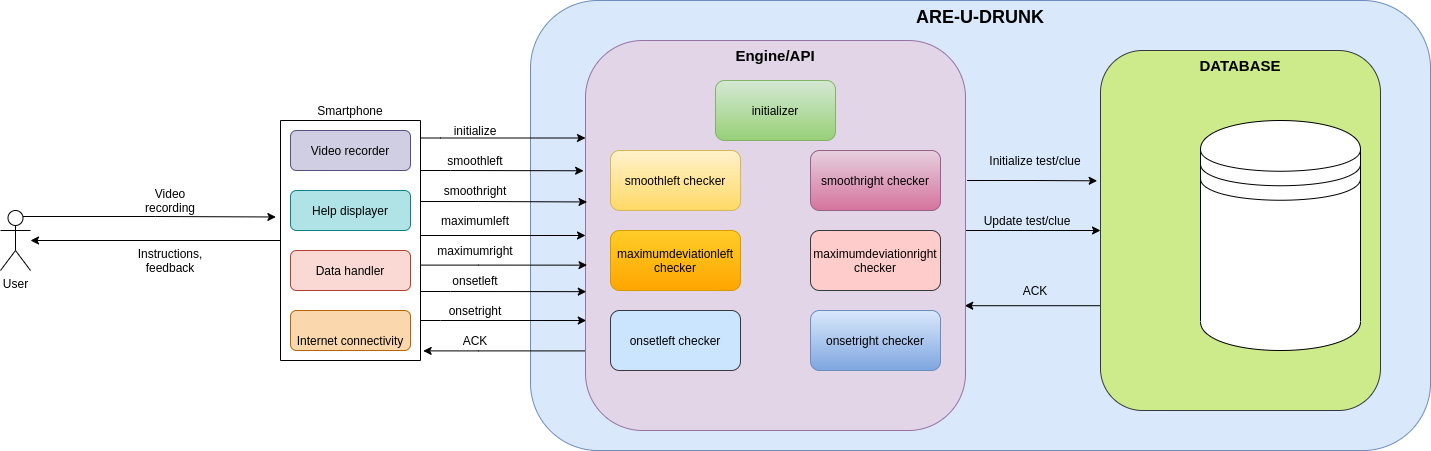
\includegraphics[angle=90, height=23cm,keepaspectratio]{./img/Architecture.png}
    \caption{Architecture of the system}
    \label{architecture}
\end{figure}



\subsubsection{Mobile application}

When designing the mobile application, the test prerequisites (pupil size and smooth gaze) are not considered because of the limitations of the current technology: the pupil size is very difficult to calculate because it depends on the distance to the camera and the angle of the face with respect to the phone. For this reason, the prerequisites are assumed to be correct and the mobile application is desinged as figure \ref{viewflow} shows.

\begin{figure}[H]
    \centering
    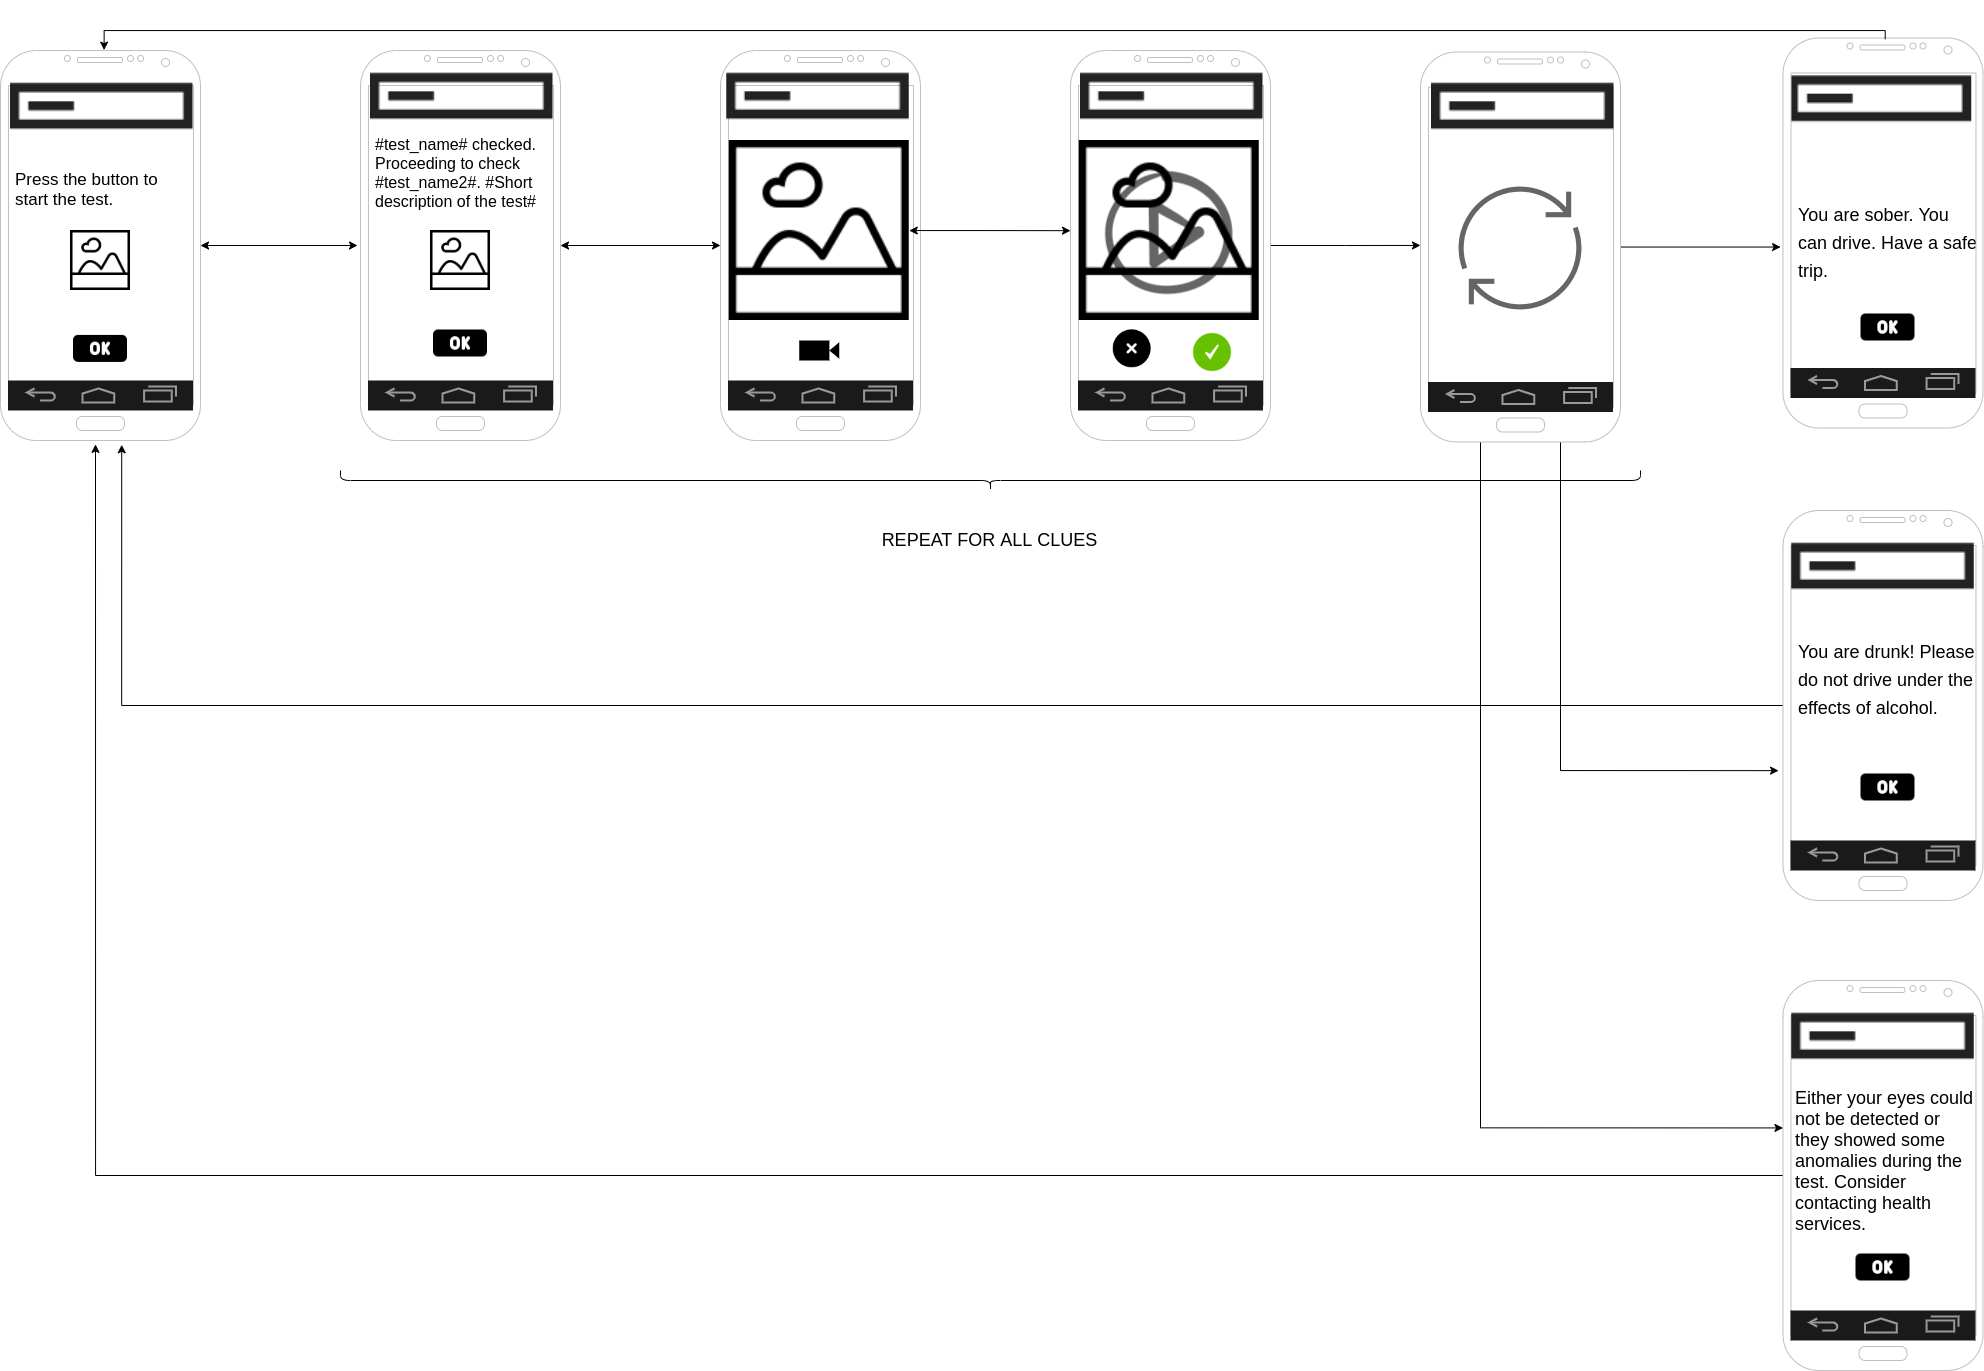
\includegraphics[angle=90, width=\textwidth]{./img/viewflow.png}
    \caption{View flow of the application}
    \label{viewflow}
\end{figure}

The application starts with a screen in which the user is informed that the test will start as soon as they click the button. Then, the user is redirected to a screen with the instructions for the clue. When pressing the camera button, the application displays a camera preview in which the user can record a video and then is redirected to a video preview where the user can confirm or discard the recorded video. In case the video is discarded, the user can record another video until the user confirms the video. This is repeated for all of the clues while less than two clues fail. If five or more clues are correct, the user is finally redirected to a screen with a success message. If two clues fail, the test stops and the user is redirected to a screen with a message encouraging the user not to drive. If the eyes are not detected in any of the clues, the test stops and the user is redirected to a screen with a message encouraging the user to reach for professional help.

Figure \ref{flowchart} shows how the user interacts with the application and the application with the server.

\begin{figure}[H]
    \centering
    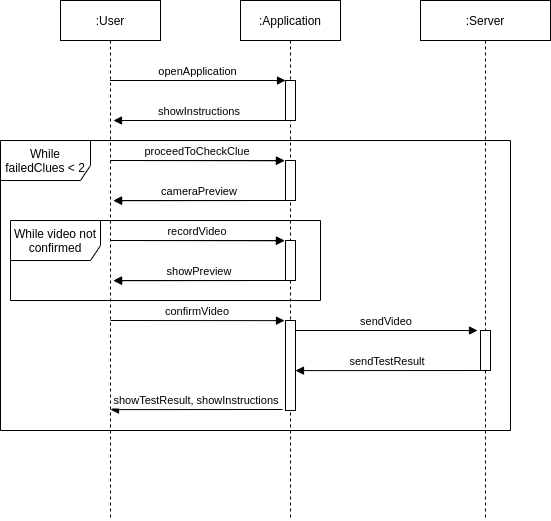
\includegraphics[width=0.95\textwidth]{./img/flowchart.png}
    \caption{View flow of the application}
    \label{flowchart}
\end{figure}

\subsubsection{Server}

The server consists on two modules: the database and an REST API that interacts with the database and the application.

The database contains relevant data about the tests and the clues, like:

\begin{itemize}
  \item Start and end timestamps of the tests.
  \item An unique user identifier.
  \item The URL where the video is stored.
  \item The type of clue.
  \item The result of the test and each of the clues.
\end{itemize}

The API receives the clues' data (videos) sent from the application. Each of the clues call their own endpoint that proccesses them to determine whether the clue is passed or failed, returns the results to the mobile application and finally creates the corresponding entries in the database, storing the video in a folder in the server. This interaction is shown in Figure \ref{architecture}.
